\documentclass[A4paper,11pt]{marine_2023_Paper}
\usepackage{graphicx}
\usepackage{amsmath}
\usepackage{amsfonts}
\usepackage{amssymb}
\usepackage{titlesec}
\titleformat{\section}[block]
{\normalfont\bfseries\filcenter}
{\thesection.}{.5em}{\bfseries}

\pagestyle{plain}



\title{Instructions to Prepare a Full Paper for the X International Conference on Computational Methods in Marine Engineering MARINE 2023}

\author{Ole Lindberg$^{1}$, Ole Vilmann$^{1*}$ and Michael Jeppesen$^{1}$}

\heading{First A. Author, Second B. Author and Third C. Author}

\address{$^{1}$ Department of Simulation, Training and Ports, FORCE Technology,
	Hjortekærvej 99, DK-2800 Lyngby, Denmark, web page: https://forcetechnology.com
	\and
	$^{*}$ Corresponding author: Ole Vilmann, ov@forcetechnology.com}

\newcommand{\V}[1]{\boldsymbol{#1}}
\newcommand{\M}[1]{\mathbf{#1}}
\newcommand{\nn}{\nonumber}
\newcommand{\D}[2]{\frac{\partial #1}{\partial #2}}

\begin{document}
\maketitle
\thispagestyle{empty}
\setlength{\parskip}{0.3cm}

\begin{center}{\bf ABSTRACT}\end{center}

Abstractttt

\noindent {\bf Keywords}: keyword 1; keyword 2; keyword 3; keyword 4; keyword 5; keyword 6.

\section*{NOMENCLATURE}

\begin{tabular}{ll}
 $C_x$ & Aerodynamic force coefficient in the $x$-direction [-]\\
 $D_{ij}$ & Shear stress tensor [Pa]\\
 $\boldsymbol{F}$ & Aerodynamic force vector [N,N,N]\\
 $F_x$ & Aerodynamic force in the $x$-direction [N]\\
 $I_{\mathrm{beam}}$ & Area moment of inertia of the beam [m${}^{4}$]\\
 $p$ & Hydrostatic pressure [Pa]\\
 $U_{\infty }$ & Free stream velocity [m s${}^{-1}$]\\
${\tau }_x$ & Skin friction in the $x$-direction [Pa]\\
 $\rho $ & Fluid density [kg m${}^{-3}$]\\
 CFD &Computational Fluid Dynamics\\
 EFD &Experimental Fluid Dynamics
\end{tabular}

\section{INTRODUCTION}

Safe and efficient navigation of large ships in shallow and confined water is a challenge. 

New container ships are enlarged to increase fuel efficiency and offshore installation vessels are larger to accommodate as many wind turbine parts as possible. 

Often these ships must navigate shallow and confined fjords or navigation channels to reach inland ports. We must ensure safe, predictable, and efficient navigation in these shallow and confined waters, and protect the marine environment in coastal areas. 

Safety is assessed by maritime engineering analysis tools and maintained by training of maritime officers in maritime simulators.

In order to address the challenges, we are developing new numerical tools for prediction of squat, bank effects and ship to ship interaction. Our goal is to accurately calculate the hydrodynamic interaction forces and moments on ships in real-time in maritime training simulators. Ships navigating in coastal and inland waterways are sailing relatively slow, hence both the length- and depth-based Froude numbers are small (< 0.2), and the well-known double body model gives a valid approximation of the hydrodynamic ship flow. We are using the state-of-the-art boundary element model pi-BEM [1] to solve the double body potential flow problem. 

pi-BEM has higher order polynomial elements, numerical quadrature for singular integrals, adaptive multi resolution quadrilateral mesh generation directly on the ships CAD geometry, fast multipole optimization of matrix vector products and MPI parallelization. 

We have extended the pi-BEM by streamlined pre-processing of the CAD geometry, developed new error-estimators for the adaptive multiresolution, developed numerical methods for calculation of flow separation along geometrical edges, compared squat prediction and bank effects with experiments for the ship models KCS and KVLCC2 [2].



bank forces and moments between our BEM model and model experiments 

assessment of navigation limits in the Limfjord in Northern Denmark.

\section{DOUBLE BODY POTENTIAL FLOW MODEL}
The hydrodynamic interaction force between a ship and other ships, the seabed, banks or fixed structures is strongly related to pressure changes due to increased or decreased flow velocity around the ship. The physical problem resembles that of a Venturi pipe. A mathematical model for calculation of a ships hydrodynamic interaction forces should capture the the Venturi pipe effect between the ships. Fortunately thats excately what the \emph{double body flow model} does. In the double body flow model is to assume that the free surface is flat and the body is mirrored the body and solution around
the still water level.
The double body flow model is based on potential flow theory, hence the water is assumed to be in-
compressible, inviscid and irrotational, and where the fluid velocity is the gradient of the velocity potential $\V{u} = \nabla \phi$. 
Mass conservation is satisfied through the Laplace equation for the velocity potential
\begin{equation}
	\nabla^2 \phi = 0, \quad z \in [-h,\eta],
\end{equation}
where $h$ is the sea depth and $z = 0$ is still water level. At the seabed the no-flux boundary condition applies
\begin{equation}
	\V{n} \cdot \nabla \phi = 0, \quad z = -h, 
\end{equation}
where $\V{n} = [n_x, n_y, n_z]^T$ is the normal vector to the seabed, pointing out of the fluid and into the seabed. Likewise are submerged bodies subject to the no-flux boundary condition
\begin{equation}
	\V{n} \cdot \nabla \phi = n \cdot \V{V} , \quad (x, y, z) \in S_B, 
\end{equation}
where $\V{n}$ is the normal vector pointing out of the fluid and into the body, $\V{V} =\V{u}_B + \V{\omega}_B \times \V{r}$ and $\V{u}_B$ and $\V{\omega}_B$ are the linear and rotational velocities of the body, $\V{r}$ is the direction vector from $CG$ and $S_B$ is the submerged surface of the body. A ship navigating in an open sea has the far-field boundary condition [9]
\begin{equation}
	\phi = \mathcal{O} (\sqrt{x^2 + y^2}) \quad \mathrm{for} \quad x^2 + y^2 \rightarrow \infty. 
	\label{eq_farfield}
\end{equation}
Conservation of momentum of a inviscid and irrotational fluid flow is described by the Bernoulli equation. In a ship fixed moving frame of reference, where the Bernoulli constant is zeros due to the far-field condition \eqref{eq_farfield}, it is
\begin{equation}
	p(x, y, z) = -\rho \left(\D{\phi}{t} -\V{V} \cdot \nabla \phi + \frac{1}{2} \nabla \phi \cdot \nabla \phi + gz \right).
	\label{eq_bernoulli}
\end{equation}
The hydrodynamic force on the submerged body is
\begin{equation}
	\V{F} = \int_{S_B} p(x, y, z) ~\V{n} dS.
	\label{eq_hydrodynamic_pressure_force} 
\end{equation}

\subsection{Linearization and Pertubation Expansion}
First we Taylor expand the velocity potential around the still water level, $z_{SWL}$,
\begin{equation}
	\phi(x,y,z) = \phi(x,y,z_{SWL}) + \eta \left.\D{\phi}{z}\right|_{x,y,z_{SWL}} + \mathcal{O}(\eta^2),
	\label{eq_phi_tay_exp}
\end{equation}
where the free surface elevation is $\eta = z-z_{SWL}$. Secondly, both the velocity potential and free surface elevation are perturbation expanded due to a small parameter $\varepsilon$
\begin{align}
	\phi = \phi_0 + \varepsilon \phi_1 + \mathcal{O}(\varepsilon^2), \label{eq_phi_per_exp} \\
	\eta = \eta_0 + \varepsilon \eta_1 + \mathcal{O}(\varepsilon^2).\label{eq_eta_per_exp}
\end{align}
Insertion of the expansions \eqref{eq_phi_tay_exp}, \eqref{eq_phi_per_exp} and \eqref{eq_eta_per_exp} in the Bernoulli equation \eqref{eq_bernoulli} and keeping only the zero'th order terms gives
\begin{equation}
	p(x, y, z) \approx -\rho \left(\D{\phi_0}{t} -\V{V} \cdot \nabla \phi_0 + \frac{1}{2} \nabla \phi_0 \cdot \nabla \phi_0 + gz \right),
	\label{eq_bernoulli_exp}
\end{equation}
and evaluation of this at the free surface, where the atmospheric pressure is assumed to be zero, and keeping only the zero'th order terms gives
\begin{equation}
	\eta_0 =  \frac{1}{g} \left(\D{\phi_0}{t} -\V{V} \cdot \nabla \phi_0 + \frac{1}{2} \nabla \phi_0 \cdot \nabla \phi_0\right).
\end{equation}
Now the surface integral for hydrodynamic force is split into the part under $SWL$ and the variation from $SWL$ due to $\eta$
\begin{align}
	\V{F} &= \int\limits_{S_{B,SWL}} p(x, y, z) ~\V{n} dS + \int\limits_{ S_B\backslash S_{B,SWL}} p(x, y, z) ~\V{n} dS.
\end{align}
The latter integral is simplified by insertion of the expanded pressure \eqref{eq_bernoulli_exp} and the vertical integration limits from $z_{SWL}$ to $z_{SWL}+\eta_0$
\begin{align}
	\V{F} &= \int\limits_{S_{B,SWL}} p(x, y, z) ~\V{n} dS + \frac{1}{2}\rho g\int \int\limits_{z_{SWL}}^{z_{SWL}+\eta_0}  \eta_{0,y<0}^2 ~dzdx- \frac{1}{2}\rho g\int\eta_{0,y>0}^2 ~ dx. \\
	\V{F} &= \int\limits_{S_{B,SWL}} p(x, y, z) ~\V{n} dS + \frac{1}{2}\rho g\int  \eta_{0,y<0}^2 ~dx- \frac{1}{2}\rho g\int\eta_{0,y>0}^2 ~ dx.
\end{align}

\section{BATHYMETRY MODEL}
Bathymetry model here understood as an interpolation of depth measurements. Harbor authorities often measure the depth in the navigation channel to the harbor regularly (multiply times per year), to know the maximum allowed ship draft for safe passage to the harbor. These depth measurements are made with sounding equipment and often presented in an uniform quadrilateral grid with e.g. $0.5$m or $1.0$m distance between the grid points. Thus, high-quality data in navigation channels are available for application in numerical models for squat and bank-effect calculations. However, the hydrodynamic pressure on ships is greatly affected by the depth outside the navigation channels, where the depth is sparsely measured. Sources for depth measurements in these areas are often limited to whats available in navigation charts or from satellite-derived bathymetry (SDB). The SDB method does not work well in deeper areas or in muddy waters where light penetration is limited. Therefor, the one often has to rely on the navigation chart. 

The interpolation point set is highly regular in some areas and sparse and scattered in other areas. Geospatial interpolation methods for scattered data like \emph{kriging} is an obvious choice. Here we have used \emph{hole filling} methods from computational geometry. 

The interpolation point set consist of soundings, coastline vertices and depth contour vertices from navigation charts and high-resolution soundings, in total scattered $N$ points
\begin{equation}
\V{x}_i = 	 \left[ \begin{matrix}
	 	x_i \\ y_i \\ z_i
	 \end{matrix} \right], \quad i=1,\ldots,N,
 \label{eq_points}
\end{equation}
where $x$ and $y$ are the horizontal UTM coordinates and $z$ is the vertical coordinate relative to the WSG 84 reference ellipsoid. The objective is to construct a fair interpolation function for the vertical coordinate $p(x,y)$ based on this point set. To construct a fair interpolation function we make a weighted least squares (WLS) fit of the point set, given by the minimization of the WLS functional (with Tikhonov regularization)
\begin{equation}
	f_{WLS} = \frac{1}{2}\sum_{i=1}^N \left(p(x_i,y_i)- z_i \right)^2 + \frac{1}{2}\lambda z_i^2 ,
\end{equation}
and minimization of the bathymetry surface bending energy, which gives a minimal energy surface (MES),
\begin{equation}
	f_{MES} = \int_{\Gamma} \kappa_1^2 + \kappa_2^2 ~dA,
\end{equation}
where $\Gamma \in \mathbb{R}^2$ is horizontal area and the $\kappa_1$ and $\kappa_2$ are the principal curvatures of the $p(x,y)$ surface. The horizontal area $\Gamma$ is subdivided into $M$ non-overlapping axis aligned quadrilaterals. On each quadrilateral the interpolating polynomial $p(x,y)$ represented two-dimensional $5^{th}$ order Bezier polynomials, here define on the unit reference square
\begin{equation}
	S(u,v) = \sum_{i=0}^n\sum_{j=0}^m B_{i,n}(u)B_{j,n}(v) p_{i,j}, \quad n=m=5, \quad 0 \leq u,v \leq 1.
\end{equation}
Since the quadrilaterals are axis aligned the mappings from the $x,y$ coordinates to the $u,v$ coordinates are univariate linear functions. Between the quadrilaterals we require $C^0$, $C^1$ and $C^2$ continuity. For the $5^{th}$ order Bezier polynomial, with $36$ degrees of freedom, that gives nine constraints for each of the four vertices in the quadrilateral, in other words we require the continuity of the derivatives
\begin{equation}
	p,~p_x,~p_y,~p_{xx},~p_{xy},~p_{yy},~p_{xxy},~p_{xyy},~p_{xxyy}
\end{equation}
at the vertices. Furthermore, we require the interpolating polynomial to bounded upwards by the still water level 
\begin{equation}
	p(x,y)< z_{SWL}, \quad x,y \in \Gamma.
\end{equation}

This bounded constrained optimization problem is formulated as 
\begin{align}
	&\min~f_{WLS} \quad \mathrm{and} \quad \min ~f_{MES} \nn \\
	&s.t. \nn	\\
	&[p]_{ij} =[p_x]_{ij}=[p_y]_{ij}=[p_{xx}]_{ij}=[p_{xy}]_{ij}=[p_{yy}]_{ij}=[p_{xxy}]_{ij}=[p_{xyy}]_{ij}=[p_{xxyy}]_{ij}=0, \nn \\
	& i=1,\ldots,K, \quad j=1,\ldots,L(i), \nn \\
	& 	p(x,y)< z_{SWL}, \quad x,y \in \Gamma.
	\label{eq_opt1}
\end{align}
where $[]$ is the jump operator, $K$ is the number of vertices and $L(i)$ is the number of element interfaces adjacent to the $i^{th}$ vertex. 

Solution of \eqref{eq_opt1} requires an minimization solver for two objective functions. Such solvers exist, but we find them to be exotic and beyond whats available in common optimization libraries. Instead we reformulate the WLS objective function into a inequality constraint. We solve the WLS problem by setting the gradient of $f_{WLS}$ with respect to $p_{i,j}$ equal to zero. In vector notation the WLS objective function is 
\begin{equation}
f_{WLS} = \frac{1}{2} (\M{A}\V{p}-\V{z})^T W (\M{A}\V{p}-\V{z}) + \frac{1}{2} \lambda \V{p}^T\V{p},
\end{equation}
and its gradient equal to zero
\begin{equation}
\V{g} = \D{f_{WLS}}{\V{p}} = \M{A}^T\M{W}\M{A}\V{p} - 2\M{A}^T\M{W}\V{z} + \lambda \V{p} = 0.
\end{equation}
Now, instead of solving the WLS problem we can formulate it as inequality constraint for the negative elementwise gradient squared
\begin{equation}
	- g_i^2 \geq 0.
\end{equation}
This will push the gradient towards zero. Now the bounded constraint optimization problem looks like this
\begin{align}
	&\min ~f_{MES} \nn \\
	&s.t. \nn	\\
	& - g_i^2 \geq 0 \nn \\
	&[p]_{ij} =[p_x]_{ij}=[p_y]_{ij}=[p_{xx}]_{ij}=[p_{xy}]_{ij}=[p_{yy}]_{ij}=[p_{xxy}]_{ij}=[p_{xyy}]_{ij}=[p_{xxyy}]_{ij}=0, \nn \\
	& i=1,\ldots,K, \quad j=1,\ldots,L(i), \nn \\
	& 	p(x,y)< z_{SWL}, \quad x,y \in \Gamma.
	\label{eq_opt1}
\end{align}
which we can solve with a standard minimization solver.

\subsection{Mesh Generation}
In this section we describe how the multi-resolution quad-tree mesh is generated which keeps a $5^{th}$ order Bezier polynomial in each element.

First we find the axis aligned bounding box of the point set \eqref{eq_points} and extend the shorter side to equal the longer side. In this square, we generate a quad-tree mesh by subdividing the tree-nodes until there is a specified number of points in each leaf-node. From this quad-tree we generate a \emph{doubly connected edge list} (DCEL). Then a Bezier polynomial is assigned to each face of the DCEL and the mesh is ready for finding a fair interpolating surface.

\subsection{Solver}
The minimization problem includes both inequality and equality constraints and solution bounds. We found that the \emph{barrier-based primal-dual interior point method} (PDIPM) available is in PETSc TAO [REF] is capable of solving this problem.

\section{VALIDATION SQUAT AND BANK-EFFECTS}
The squat calculation of the double body $\pi$-BEM has been extensively validated in [MASHCON REF]. Comparing to the shallow water experiments published in SIMMAN 2013, for both the KCS and KVLCC2 models, we found that sinkage is accurately predicted for moderate depth Froude numbers $Fr_h<0.2$. 

The sway force on KVLCC2 due to the presence of a vertical wall was also calculated in [MASHCON REF] and found to be mainly between the EFD sway forces obtained with and without propulsion, respectively. This was a hint that the sway force calculation was satisfactory, but more detailed validation is needed for sloping banks both with and without surface penetrating of the bathymetry. We anticipated examination of the sway and yaw force against the bank-effect experiments published in [ref MASHCON 2009], but have realized that these experiments are for relatively high depth Froude numbers $Fr_h$ and that the published experiments are simply to few for meaningful comparison. To our knowledge, there are no other open data publications with bank-effects for sloping banks, so hopefully we will be able to make the necessary experiments or more open data on bank effects will be published in the future.  

\section{APPLICATION: NAVIGATION ON LIMFJORDEN}
Limfjorden is a fjord in northern Denmark that cuts through Jutland from the North Sea in west to Kattegat in east. Port of Aalborg is an inland harbor located in the eastern part of Limfjorden approximately $10$ nm from Kattegat. The renewable energy industry in Aalborg depends on safe maritime transport on Limfjorden with e.g. large offshore supply ships.

We are building the bathymetry model based on high-resolution ($1$m$\times$$1$m) soundings in the navigation channel, sounding from the navigation chart and vertices from $0$m, $2$m, $6$m and $10$m depth contours. The number of high-resolution points in the navigation channel is $5746216$ and the number of sounding points and contour vertices are $4089$. A total $5750305$ points. The scattered point set is seen in figure \ref{fig:screenshot-from-2023-04-17-20-23-15}.

\begin{figure}
	\centering
	\includegraphics[width=1.0\linewidth]{"Screenshot from 2023-04-17 20-23-15"}
	\caption{}
	\label{fig:screenshot-from-2023-04-17-20-23-15}
\end{figure}

The axis aligned bounding box for the quad-tree generation covers an area of $21.287$km $\times$ $21.287$km. The maximum depth of the quad-tree is $8$ and the maximum number of points per leaf node is $2$. The resulting quad-tree has $3886$ leaf nodes. From the quad-tree we build a DCEL mesh, with $3886$ vertices and $3254$ faces, which is seen in figure \ref{fig:screenshot-from-2023-04-17-20-43-40}. 

\begin{figure}
	\centering
	\includegraphics[width=1.0\linewidth]{"Screenshot from 2023-04-17 20-43-40"}
	\caption{}
	\label{fig:screenshot-from-2023-04-17-20-43-40}
\end{figure}

\begin{figure}
	\centering
	\includegraphics[width=0.7\linewidth]{"Screenshot from 2023-04-17 21-43-39"}
	\caption{}
	\label{fig:screenshot-from-2023-04-17-21-43-39}
\end{figure}

\begin{figure}
	\centering
	\includegraphics[width=0.7\linewidth]{"Screenshot from 2023-04-17 21-41-58"}
	\caption{}
	\label{fig:screenshot-from-2023-04-17-21-41-58}
\end{figure}

\subsection{Tables}

 Tables are numbered consecutively and captioned. The caption title is bold followed by full stop (e.g. \textbf{Table~1}), all caption is 11 points and centered above the table.

 The body of the table is 11 points. Tables are positioned within the body of the article, centered, and as close as possible to the place where they are first discussed. Bold and colored shading can be applied.

 \begin{table}[h!]
\caption{This is an example of a table showing the template margins.}
\begin{center}
\begin{tabular}{{l}p{0.2in}{l}}
Top & &2.5 cm \\
Bottom && 2.5 cm \\
Left && 2.0 cm \\
Right && 2.0 cm \\
Gutter && 0.0 cm \\
Header && 1.0 cm \\
Footer && 1.0 cm \\
\end{tabular}
\end{center}
\end{table}

\begin{table}[h!]
\caption{Page numbers format.}
\begin{center}
\begin{tabular}{lp{0.2in}l}
Position & &Bottom of the Page \\
Alignment & &Center \\
Number on first page && Yes \\
First page number && 1 \\
\end{tabular}
\end{center}
\end{table}

\subsection{Figures}

 The Author should make every effort to include figures of memory size small enough so that the document size is manageable for downloading and opening over the internet and, at the same time the resolution of the figures is adequate for printing.

 All figures should be numbered consecutively and captioned. The caption should be 11 point bold, placed below the figure (as opposite to table captions that are placed above the table).

 Figures should be positioned within the body of the article, centered, and as close as possible to the place where they are first discussed. Wrapping style should be ``in line with text''. Color graphs, photos and animations are encouraged.

 IMPORTANT: text within the figure should be no smaller than 9 points, and the symbols should appear with the same font type as in the Nomenclature.

 Equations, figures and tables can be referenced in the text such as, for instance, equation 1, Eq. 1, Eqs. 1 and 2, Eqs. 1-3, Fig. 1, Figs. 1a and 1b (for multiple sub-figures), Tab. 2, \textit{etc. }

 When necessary, use Column Break to keep the caption with its table or figure on the same page.

\begin{figure}[t]
\centering
%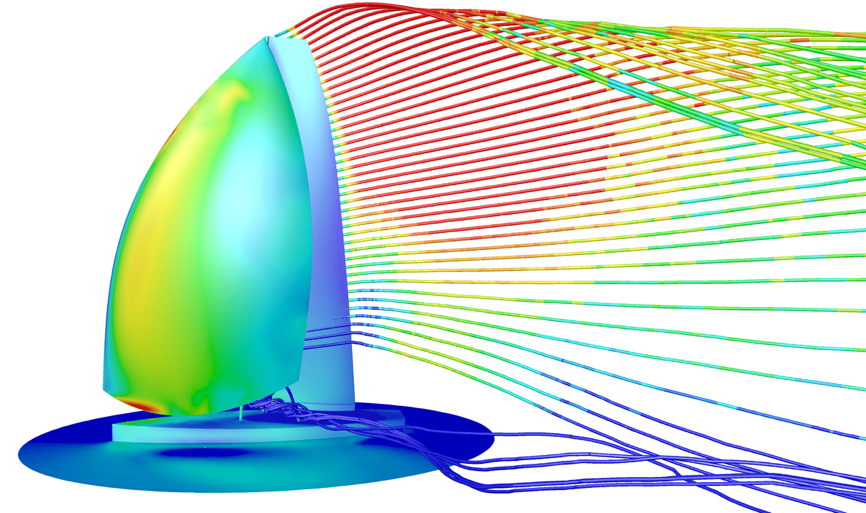
\includegraphics[width=11cm]{fig-example.eps}
\caption{Example of a figure.}
\label{fig1}
\end{figure}

\subsection{Citations}

 When the citation is part of the sentence, the citation includes the Author's last name and, between parentheses. For example, Bowman (1988) showed that this is a good citing style. Conversely, when the citation is not part of the sentence, then also the Author's name is within parentheses  (Bowman, 1988). Append lower-case letters to the year in cases of ambiguity (Bowman, 1989a). Multiple Authors are treated as Bowman and Skipper (1988) when there are two Authors and, in the case of three or more Authors, we list only the first Author followed by \textit{et al. }in italic. For example, see Bowman \textit{et al.} (1988). Multiple citations that are not part of the sentence should be separated by semicolons  (Bowman 1989; Skipper 1990).

\subsection{Inquiries}

 If you have any questions about the preparation or submission of your article as instructed here, please send an email to marine@cimne.upc.edu.

\section{DISCUSSION}
Bathymetry model kriging 
% 	https://help.arcgis.com/en/arcgisdesktop/10.0/help/index.html#//009z00000076000000.htm
% https://www.publichealth.columbia.edu/research/population-health-methods/kriging-interpolation


\section{CONCLUSIONS}

 It is recommended that the main body of the text ends with a summary of the key conclusions. This section may include a summary of the scope and of the methodology of the article, and a detailed list of conclusions in order of importance.

\section*{ACKNOWLEDGEMENTS}

 Every fund that supported the research must be acknowledged. Brief personal acknowledgements may also be added. For example, ``this work received funds from the European Research Council (grant no. XXXXXX). The authors are especially grateful to the Reviewers for their help in improving the article. This section can be skipped if the research has not received any financial contribution.

 \section*{AUTHOR'S CONTRIBUTION}

 This section is not compulsory. Authors can consider to identify their contribution to the reaserach project and the preparation of the manuscript. Example text is as follow. ``FAA designed the experiments, processed the data, and wrote the first draft of the manuscript. FAA and SBA undertook the experiments and processed the data. TCA supervised and coordinated the project. All authors edited and approved the manuscript.''


\section*{REFERENCES}
All references cited in the text should be listed at the end of the article in alphabetical order.

Bowman, A. B. (Year). Book Title (italic, initial capitals followed by lower case on all words except articles, conjunctions, and prepositions, which should appear entirely in lower case). Publisher, city, country.

Bowman, A. D. and Skipper, E. F. (Year). Title of Journal Article (roman font, initial capitals followed by lower case on all words except articles, conjunctions, and prepositions, which should appear entirely in lower case). Journal Name (in italic), volume (number), pages.

Bowman, A. D. and Skipper, E. F. (1988). Title of Journal Article. Journal of Sailing Technology, 2, 1-31.

Bowman, A. D., Skipper, E. F. and Pitman, J. K. (Year). Title of Conference Article. Proceedings of Conference Name (in italic), dates, city, country.

Bowman, A. D., Skipper, E. F. and Pitman, J. K. (1988). Title of Conference Article. Proceedings of Conference Name, March 15-16, Annapolis, MD, USA.

Larsson, L., Eliasson, R. and Orych, M. (2014). Principles of Yacht Design. Adlard Coles Nautical, London, UK.

\end{document}


